\chapter{Mathematical Model}

\addcontentsline{toc}{chapter}{Mathematical Model Development}

\section{Model Description}

We are going to observe a mathematical model proposed by \cite{lips}, which describes the epidemiology of antimicrobial resistant infections in hospitals. The model examines a population of people in a closed environment, where new patients come into the system at some rate and go out of the system respectively. The model can be applied for the diseases that are transmitted through the skin, respiratory or digestive organs. A few examples of such bacteria are Escherichia coli, Staphylococcus, Enterococcus, Klebsiella pneumoniae and others. The mentioned bacteria are dangerous enough to cause a painful or even lethal infection. The hospital environment was chosen because the transmission of these bacteria often takes place inside the hospitals. Different patients may accidentally contact with each other and spread their infections to one another, as well as to medical personnel. The medical workers are also often responsible for the spread of infections inside the hospital, since they may pass the bacteria between their patients. This might happen as a result of insufficient hygiene with respect to their hands and inventory items. The bacteria in the system are continuously encountering the antibiotics that are used in the hospital. As a result, the patients may always get infected accidentally and the bacteria can pass their antibiotic resistant plasmids to other strains.

The model observes the transmission dynamics of the bacteria in a hospital, with regard to the usage of two different antibiotics - drug A and drug B. Some portion of all individuals that enter the hospital are already colonized with the bacteria, that we are looking at. The differential equations for the model will look as follows:

\begin{equation}
\frac{dS}{dt} = m \mu + \beta S X - (\tau_1 + \tau_2 + \gamma + \mu) S
\end{equation}

\begin{equation}
\frac{dR}{dt} = \beta (1 - c) R X - (\mu + \tau_2 + \gamma) R
\end{equation}

\begin{equation}
\frac{dX}{dt} = (1 - m) \mu + (\tau_1 + \tau_2 + \gamma) S + (\tau_2 + \gamma) R - \beta S X - \beta (1-c) R X - \mu X.
\end{equation}

$S$ in the equations, denotes the individuals that are infected with the bacteria sensitive to drug A. $R$ is correspondingly stands for the population infected with the bacteria resistant to drug A. By $X$ we denote the people who are not carrying any type of these bacteria. Also, it is assumed that there are no any bacteria resistant to drug B in the system. A fraction $m$ of people entering the bacteria is infected by a sensitive strain; the other $1-m$ of incoming people are not colonized with the bacteria at all ($X$).

\section{Model Implementation Platform}

AnyLogic is a multi-method simulation modeling tool developed by XJ Technologies.
The tool was named AnyLogic, because it supported all three well-known modeling approaches: System dynamics, Discrete event simulation, Agent-based modeling.

AnyLogic models can be based on any of the main simulation modeling paradigms:discrete event or process-centric (DE),systems dynamics (SD), and agent-based(AB)

\begin{figure}
   \centering
	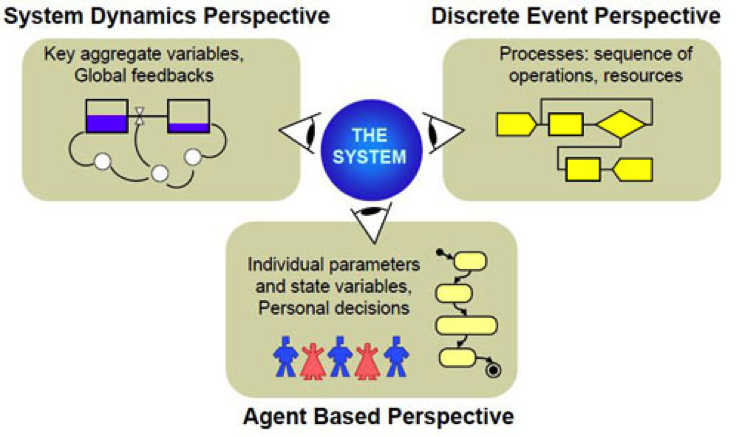
\includegraphics[width=0.9\textwidth]{img/system}
	\caption[Clear]{Modeling aproaches}
\end{figure}

System dynamics and discrete event are traditional simulation approaches, agent based is new. Technically, the system dynamics approach deals mostly with continuous processes whereas "discrete event" (by which we mean all descendants of GPSS also known as process-centric simulation approach) and agent based models work mostly in discrete time, i.e. jump from one event to another.

System dynamics and discrete event simulation historically have been taught at universities to very different groups of students, namely management and economy, industrial and operation research engineers. As a result, there are two distinct practitioners' communities that never talk to each other.

Agent based modeling until recently has been mostly a purely academic topic. However, the increasing demand for global business optimization caused leading modelers looking at combined approaches to gain a deeper insight into complex interdependent processes having very different natures.

AnyLogic includes a graphical modeling language and also allows the user to extend simulation models with Java code. The Java nature of AnyLogic lends itself to custom model extensions via Java coding as well as the creation of Java applets which can be opened with any standard browser. These applets make AnyLogic models very easy to share or place on websites. In addition to Java applets the Professional version allows for the creation of Java runtime applications which can be distributed to users. These pure Java applications can be a base for decision support tools System dynamics dealing with aggregates is obviously used at the highest abstraction level. Discrete event modeling is used at low to middle abstraction. As for agent based modeling, this technology is used across all abstraction levels, and agent may model objects of very diverse nature and scale: at the "physical" level agents may be e.g. pedestrians or cars or robots, at the middle level – customers, at the highest level – competing companies.

AnyLogic allows the modeler to combine these simulation approaches within the same model. There is no fixed hierarchy. So, as an example, one could create a model of the package shipping industry where carriers are modeled as agents acting/reacting independently whereas the inner workings of their transport and infrastructure networks could be modeled with discrete event simulation. Similarly, one can model consumers as agents whose aggregate behavior feed a systems dynamics model capturing flows such as revenues or costs which do not need to be tied to individual agents. This mixed language approach is directly applicable to a wide variety of complex modeling problems that may be modeled via any one approach albeit with compromises.


\section{System Dynamics Based Stochastic Modeling}

System dynamics models are becoming increasingly common in the analysis of policy and managerial issues. The usefulness of these models is predicated on their ability to link observable patterns of behavior to micro-level structure and decision-making processes.

Since its inception, system dynamics (SD) has emphasized the importance of clarity of purpose for any intervention––a defined problem, issue or undesirable behavior to be corrected (Forrester,1961). The problem behavior is usually described in a reference mode, and the purpose of the intervention is to identify how structure and decision policies generate the identified reference mode so that solutions can be generated and implemented.

SD practitioners build and depend on formal simulation models to overcome the cognitive limitations to grasp the de tailed complexity of the problem situation, an d to make reliable behavioral inferences. Generation of problem solutions relies on using these models for policy testing (Forrester, 1961), what -if scenarios (Morecroft, 1988), or policy optimization (Kleijnen, 1995). All of these efforts, however, presume confidence that the model represents the structure of the problem situation and that his structure is responsible for the observed behavior.

We see that there are Projects panel where projects are viewed, Palette panel where the elements of the modeling are stored and on the bottom side Description panel that specifies the properties for the components of the model. And the main panel where the models are built.

When constructing the model on Any Logic, we use stocks and flows diagram. Stock is something like a container which stores the values and can receive inputs and give values for outputs. Flow describes the transitions from one state to another, from one stock to another. After adding stocks and flows, we add the variables that were specified in the model. Then we link the auxiliary variables to the stocks and flows. By linking we mean that a variable impacts the flow or stock.


% part II
On the basis of the mathematical model which I developed in previous section, I add a stock with susceptible people and then draw 5 flows going from Susceptible to Exposed state.  It means that I divide the population into 5 categories. So, 5 flows describe transitions and infection rates of each category. For each infection rate, there are special variables that impact on them. Looking at the formula 1.1 I see that 2 variables affect the equation. They are contact rate and infectivity. So, I link them to the flow and write the equation. Each flow has its own contact rate and infectivity.

Contact Rate has a random nature. It is the average number of contacts of infected person per day. I take the randomness of contact rate because I consider that obviously person can change the number of contacts per day. When writing the equation for this parameter I use triangular distribution. As we can see, C5 is the parameter that defines the contact rate for 5th category that is elder people aging from 60 and older. On the Properties panel I write the equation for the variable – triangular (6,15). It means that elder person contacts minimum with 6 and maximum with 15 individuals per day. I assume that older person usually doesn’t work and sits at home, he/she has limited number of contacts.

Such definition of parameters was done for other categories too. For the 1st category (babies between 0-2 ages) I took the contact rate between 3 and 7 people. I wrote the equation as triangular (3,7). This is due to the fact that babies see only their family and nobody else. And in average there’s 4 -5 people in family. For the 2nd category with ages 3-6, contact rate is between 10 and 20. I took into account that kids of these ages usually go to kindergartens where there are many kids around 15 people. For the 3rd category with ages 7-18, contact rate is lies between 20 and 30. These are the teenager who go to school and meet with friends, and as we know in the school in one class there are about 25 people. For the 4th category with ages 18-60, they are assumed as workers, employees who can go anywhere. So their contact rate is pretty high also because at the workplace there can work hundreds of people. Their contact rate is also between 20 and also. In fact these assumptions can change based on the situation. So there are no definite and exact numbers.

Infectivity has also random nature between 0 and1. This variable defines the probability of one person getting the disease with one contact per time. So, it depends on the immunity of individual. I take also triangular distribution for this variable. As we can see, I set the infectivity for the 1st category kids of ages 0-2. Usually, newborn kids have immunity from their mother but at the same time they are vulnerable, too. So, their infectivity is in average 0.4.

The same actions are applied to other categories. For the children with ages 3-6, the infectivity is 0.5 as they are young and strong. The distribution function is triangular (0,1,0.5). So, they are not likely to get the disease first. For the 3rd category with ages 7-18, the infectivity is on average 0.3 because of their age. For the 4th category as employees and students, the infectivity is 0.4. And the last is the most vulnerable category that is elders. As it’s known, older people has weak immunity. So, they are the most who suffer from flu actually. Therefore, their infectivity is high – 0.8.

After we set the values for parameters, we write the equations for the flows which define the transition from one state to another. First, we write the infection rates for each category. It is the equation for the elder people. C5 is contact rate, I5 is infectivity, Infected Population is the sum of infected people from each category.  Total Population *0.09 means that elder people form 9\% of our population. It’s based on the statistical data.
